\chapter{Introduction}

Nearly all life on Earth exists in a temporally periodic environment.
The 24-hour day-night cycle brings with it a wide variety of cyclic effects, including changes in temperature, light, and radiation.
Circadian rhythms function as a biological feed-forward controller, adapting the physiology and behavior of an organism to these predictable changes in its environment.
Endogenous circadian rhythms have been observed in nearly all species, from simple prokaryotic cyanobacteria, to plants, insects, and mammals \cite{Ishiura1998, McClung2006a, Glossop1999, Ko2006}.
While the genetic mechanism controlling these rhythms varies, circadian rhythms share three characteristics: they are endogenous, they are temperature-compensated, and they are entrainable \cite{Dunlap2004}.
Importantly, the endogenous or self-sustaining nature of circadian rhythms indicates that they are not merely responses to environmental cues, but instead are generated by underlying biological processes.

Circadian rhythms are thought to have first evolved to protect metabolites in simple organisms from harsh solar ultraviolet radiation \cite{Nikaido2000}.
In complex organisms, circadian rhythms control gene expression across a wide portion of the genome.
Approximately 10\% of all transcripts expressed in human tissue are circadian-regulated, affecting nearly every biochemical pathway \cite{Lowrey2004}.
As such, circadian regulation impacts many biological processes including cell cycles, body temperature, metabolism, insulin sensitivity, and activity patterns \cite{Refinetti1992, Bieler2014, Sassone-Corsi1998, Bass2010}.

Developing a quantitative understanding of circadian rhythms is desirable from both a medical and an engineering perspective.
With the emergence of a 24-hour society, perturbations to natural circadian rhythms are common.
Chronic disturbances, such as shift work, have been associated with metabolic disorders \cite{Haus2006}.
Irregular circadian rhythms have also associated with neurodegenerative and psychiatric disease \cite{Wulff2010}.
Additionally, due to metabolic differences, medicines taken at different phases of the circadian cycle differ in effect or effectiveness.
Medically, it is desirable to develop pharmacological or therapeutic interventions to strengthen circadian rhythms and improve overall health.
To do so requires a strong understanding of the circadian clock.
For an engineering standpoint, the circadian network is a complex yet precise gene network.
Understanding how these networks are organized is desirable in order to create synthetic genetic networks for genetic engineering.
The circadian system provides an interesting and physiologically-relevant case study for a mathematical understanding of gene networks.

\section{Organization of Mammalian Circadian Rhythms}
Circadian rhythms are generated at a single-cellular level, and are considered to be cell-autonomous.
In multicellular organisms, cell-autonomous clocks must interact at tissue and system levels to establish a coherent phase across the organism.
For mammals this task is accomplished by a ``master clock,'' the suprachiasmatic nucleus (SCN) \cite{Welsh2010}.
The SCN is a small region of the hypothalamus, consisting of approximately 20,000 neurons.
It receives light input from the optic chasm to entrain to external day-night cycles.
Signals from the SCN synchronize peripheral cellular oscillators which control gene expression in tissues throughout the body.

\subsection*{Single-Cell Rhythms}
The mammalian cell-autonomous circadian oscillator is comprised of interlocking genetic transcription-translation feedback loops (TTFLs), as shown in Fig. \ref{fig:ko-takahashi-2006} \cite{Ko2006}.
The central negative feedback loop driving rhythmicity is the \textit{Period-Cryptochrome} (\textit{Per-Cry}) loop, in which \textit{Per} and \textit{Cry} are transcribed and translated, form heterodimers, and re-enter the nucleus to repress their own transcription through sequestration of CLOCK-BMAL1 Enhancer box (E-box) activators. 
PER-CRY heterodimers are then slowly degraded \cite{Hirota2012a}.
As transcription repressors are degraded, transcription re-activates, creating a cycle with a period of approximately 24 hours.
Clock-controlled genes are then regulated by participants in this core loop, through transcription regulators including E-boxes, DBP/E4BP4 binding elements (D-boxes), and RevErbA/ROR binding elements (RREs) \cite{Ueda2005}.
This circadian network has been identified in many cell types including fibroblast, adipose, neuronal, liver, and skeletal cells \cite{Ando2005,Liu2007,Lamia2009,Zambon2003}.

Despite this complex systems of feedback loops, single cells do not oscillate with precise rhythms \cite{Barkai2000, Herzog2004}.
Rather, extrinsic and intrinsic cellular noise lead to variability in period length at a single-cell level \cite{Scott2006}.
Extrinsic sources of noise include environmental conditions and differences in the physical makeup of each cell. 
Intrinsic sources of noise include low copy numbers of oscillator components and diffusion of biochemical species within the cell.
Because each cell within an organism is individually ``sloppy,'' synchronization between cells and an organizational hierarchy is required to achieve precise rhythms at an organism-level.

\begin{figure}[htb] 
    \begin{center}
        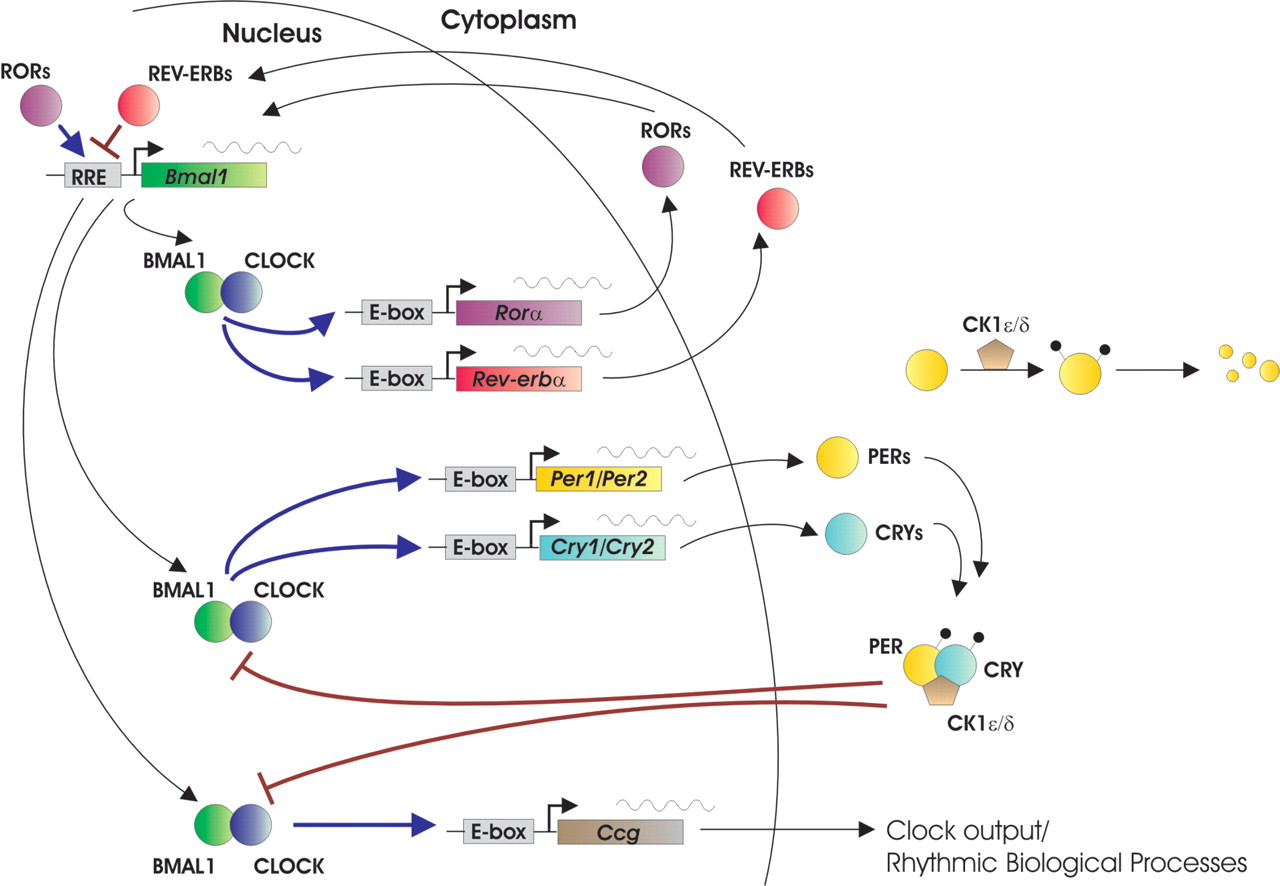
\includegraphics[width=0.85\textwidth]{intro/figures/ko-takahashi-2006.jpg}
    \end{center}
    \titlecaption{\label{fig:ko-takahashi-2006}The mammalian cell-autonomous circadian clock}{The mammalian clock is comprised of interlocking genetic feedback loops. The core negative loop is the \textit{Per-Cry} loop. \textit{Ccg} represents a family of clock-controlled genes, here symbolically controlled by an E-box region. Figure from \cite{Ko2006}.}
\end{figure}



\subsection*{Organism-Wide Rhythms}
In the suprachiasmatic nucleus, cells exchange neuropeptides, including VIP, AVP, and GABA, to maintain synchrony of the oscillator population \cite{Aton2005a, Welsh2010}.
Fig. \ref{fig:welsh-takahashi-kay-2010} shows many of the signaling pathways thought to play a role in maintaining synchrony in the SCN.
Explanted SCN maintain precise rhythms for over a month when plated in the absence of any external cues.
Oscillators in peripheral tissues are thought to lack paracrine signaling, and as such do not maintain coordinated rhythms in the absence of an entraining signal.
Entraining cues from the SCN as well as time-dependent feeding, rather than intercellular coupling, are required to maintain precise, coordinated rhythms in peripheral tissue.
Likewise, destruction of the SCN in otherwise-healthy animals results in loss of rhythmic behavior, while SCN transplants restore rhythms across the organism \cite{Silver1996}.


\begin{figure}[htb] 
    \begin{center}
        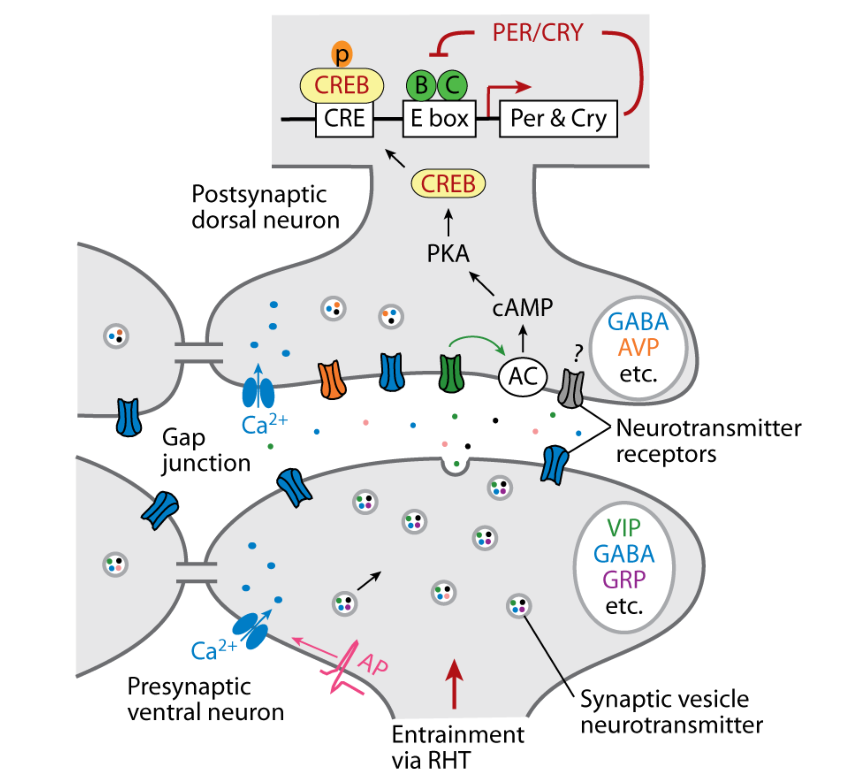
\includegraphics[width=0.55\textwidth]{intro/figures/welsh-takahashi-kay-2010.pdf}
    \end{center}
    \titlecaption{\label{fig:welsh-takahashi-kay-2010}Intercellular signalling pathways in the suprachiasmatic nucleus}{Figure from \cite{Welsh2010}.}
\end{figure}

\section{Mathematical Approaches}
The inherent complexity in circadian genetic networks necessitates a quantitative approach to understanding the underlying dynamics.
Dynamics of gene expression are frequently modeled using ordinary differential equation (ODE) approaches.
When coupled, these systems of ODEs can be used to represent and understand complex genetic networks.
Historically, ODE modeling is a well-established approach to understanding circadian rhythm dynamics \cite{Leloup2003a, To2007, Rust2007, Mirsky2009b}.
ODE models are of the form:
\begin{equation}
    \label{eqn:ode}
    \frac{d\mathbf{x}}{dt} = \mathbf{f}(\mathbf{x}(t),p),
\end{equation}
where $\mathbf{f}$ is comprised of rate equations for biochemical states $\mathbf{x}$, and is parameterized by $p$.
It is also common to treat the circadian gene network as an attractive \textit{limit cycle oscillator}, in which Eqn. \ref{eqn:ode} satisfies:
\begin{equation}
    \label{eqn:lco}
    \lim_{t\to\infty} [\mathbf{x}(t) - \mathbf{x}(t+\tau)] = 0
\end{equation}
indicating that concentrations $\mathbf{x}$ oscillate with period $\tau$.
ODE models are easily constructed, but are not easily parameterized as limit cycle oscillators.
While highly useful, ODE approaches cannot capture intrinsic molecular fluctuations which play an important role in circadian behavior.

Stochastic approaches, through Gillespie (or kinetic Monte Carlo) algorithms, are computationally expensive, but directly capture intrinsic molecular noise due to low copy numbers.
Stochastic approaches have also been previously applied to circadian rhythms at a single-cell level \cite{Forger2005, Meeker2011a}.
Rather than using a deterministic set of rate equations, stochastic simulation algorithms solve the chemical master equation (CME), of the form:
\begin{equation}
    \label{eqn:ssa}
    \frac{d\mathbf{s}}{dt} = \mathbf{A}(t)\mathbf{s},
\end{equation}
where $\mathbf{s}$ is a vector of $n$ states $s_i$ and $\mathbf{A}$ is an $n \times n$ matrix of propensities.
As $\mathbf{A}$ may depend on $\mathbf{s}(t)$, the resulting Markov process is nonstationary.

For this work, both ODE and stochastic approaches will be used, as they are each suitable for specific situations.
Additionally, understanding circadian data requires mathematical tools from a variety of fields, including sensitivity analysis, discrete signal processing, and statistics; these methods will be introduced \textit{ad hoc}.

\section{Biological Methods}
This project is purely computational, however mathematical understanding necessitates understanding of experiment.
Aside from common biological techniques, circadian research often uses the \textit{Period2::Luciferase} bioluminescent reporter to observe circadian gene expression \cite{Yoo2004}.
This fusion allows the real-time observation of \textit{Period} production in individual cells and also in cells within a tissue.
\textit{Per2::Luc} bioluminescence traces are used extensively to monitor single-cell rhythms in Sections \ref{ssec:coupled-model} and \ref{ssec:network-inference}.

\section{Significance Within Chemical Engineering}

Chemical engineering is based on the fundamental principles of thermodynamics, transport phenomena, and reaction kinetics.
This proposed thesis is not constrained to those topics alone, but is grounded in them.
Most prominently, the equations describing genetic network dynamics are equivalent to, and based on, chemical kinetic equations.
The rate equations governing biochemical species take familiar forms: mass-action, Michaelis-Menten, and Hill type kinetics.
Mathematically, these equations may be solved identically to the more traditional reactor design equations.
Here, control theory can be applied as well--concepts such as frequency domain analysis and transfer function model representations may yield significant insight into the dynamics of biochemical pathways.
When these systems of reactions are broken down into stochastic processes, statistical mechanics concepts apply as well.
The Gillespie algorithm, commonly used in stochastic systems biology, is effectively a kinetic Monte Carlo scheme \cite{Gillespie1977}.
As in statistical mechanics, fluctuations can play a significant role in system behavior, leading to dynamics that cannot be well-approximated by deterministic solutions.

Transport phenomena plays a significant role in intra- and intercellular movement of biomacromolecules.
To this point, mathematical research in circadian biology has primarily considered the interior of the cell to be spatially homogeneous.
While this is physically incorrect, it is a useful approximation.
Future models may account for transport between compartments of the cell with simple rate equations, using either partial differential equation or spatial stochastic solvers \cite{Drawert2012}.
A strong understanding of diffusive processes can assist in determining the validity of these approximations and building physical understanding of cellular dynamics.
Although intercellular transport is thought to be primarily synaptic, diffusive connections are thought to be the primary communication between the SCN and peripheral oscillators \cite{Silver1996}.

Mathematics from chemical engineering may also arise unexpectedly.
For example, the phase of uncoupled stochastic oscillators was recently captured with a reaction-diffusion equation \cite{StJohn2014b}.


